\documentclass[12pt]{article}

\usepackage[utf8]{inputenc}
\usepackage{geometry}
\geometry{a4paper,scale=0.75}
\linespread{1.5}
\usepackage{graphicx} 
\usepackage{float} 
\usepackage{subfig} 
\usepackage{enumerate}
\usepackage{enumitem}
\usepackage{amsmath}
\usepackage{array}
\usepackage{booktabs}
\usepackage{multirow}
\usepackage{amsfonts}
\usepackage[english]{babel}
\usepackage{amsthm}
\usepackage{dcolumn}
\usepackage{multicol}
\usepackage{stfloats}
\usepackage{lscape}
\usepackage[figuresright]{rotating}
\RequirePackage{pdflscape}
\usepackage[toc,page]{appendix}
\usepackage{geometry}
\usepackage{longtable}
\usepackage{comment}
\usepackage{xcolor}

% -------- enumerated sub-labels (a), (b), … --
\usepackage{enumitem}
\setlist[enumerate,1]{label=(\alph*),ref=\alph*}
% ---------------------------------------------

\usepackage{hyperref}
\hypersetup{hidelinks,
	colorlinks=true,
	allcolors=black,
	pdfstartview=Fit,
	breaklinks=true}
\usepackage{csquotes}
\usepackage{natbib}
\bibliographystyle{apalike}
\newtheorem{definition}{Definition}
\newtheorem{theorem}{Theorem}
\newtheorem{proposition}[theorem]{Proposition}
\newtheorem{lemma}[theorem]{Lemma}
\newtheorem{corollary}[theorem]{Corollary}
\newtheorem*{remark}{Remark}
\newtheorem{example}{Example}
\newtheorem{exercise}{Exercise}
\newtheorem{assumption}{Assumption}[section] % number within sections


\begin{document}

\begin{center}
    ECON 3123: Macroeconomic Theory I\\
    {\large \textbf{Tutorial Note 2: Consumption and Goods Market}}\\
    Teaching Assistant: Harlly Zhou
\end{center}

\subsection*{Decomposition of GDP}
GDP is the sum of consumption, investment, government spending, net export, and inverntory investment, which we always ignored due to its relatively tiny size.
\begin{align*}
    Y = C + I + G + NX,\,\,\,\, \text{where } NX = EX - IM.
\end{align*}
\begin{enumerate}[label=(\arabic*)]
    \item Consumption ($C$) is the purchase of goods and services by consumers. It is the largest component of GDP.
    \item Investment ($I$) is the sum of nonresidential investment (\textit{e.g.,} a new machine bought by firm) and residential investment (\textit{e.g., }purchase of a new house). 
    \item Government sepnding ($G$) is the purchase of goods and services by different layers of government. Note that government transfer is not government spending.
    \item Exports ($EX$) are purchase of domestic goods by foreigners. Imports ($IM$) are purvchases of foreign goods by domestic consumers, firms and government. Net exports ($NX$) is the difference between exports and imports. It can be negative. 
    \item Invertory investment is the difference betwee nproduction and purchases. It can be negative.
\end{enumerate}

\begin{exercise}
    \begin{enumerate}[label=(\arabic*)]
        \item Which of the following is not a category of consumption spending in the national income accounts?
        \begin{enumerate}[label=\Alph*.]
            \item Consumer durables
            \item Nondurable goods
            \item Services
            \item Housing purchases
        \end{enumerate}
        \item In the expenditure approach to GDP, which of the following would be excluded from measurements of GDP?
        \begin{enumerate}[label=\Alph*.]
            \item Government payments for goods produced by foreign firms
            \item Government payments for goods produced by firms owned by state or local governments
            \item Government payments for welfare 
            \item All government payments are included in GDP.Housing purchases
        \end{enumerate}
    \end{enumerate}
\end{exercise}

\subsection*{Consumption and Keynesian Cross}
\paragraph{Consumption Function}
The main factor that determines consumption is \textbf{disposable income}, denoted by $Y_D$. It is the income that remains once consumers receive transfers from the government and pay their taxes:
\begin{align*}
    Y_D = Y - T.
\end{align*}

We assume that the consumption satisfies the following linear relation:
\begin{align*}
    C = c_0 + c_1 Y_D = c_0 + c_1 (Y-T).
\end{align*}
This is a behvioral equation. 
\begin{enumerate}
    \item The parameter $c_0$, autonomous consumption, captures the consumption when $Y_D=0$: subsistence level of consumption, and effects of other factors.
    \item The parameter $c_1$, marginal propensity to consume (MPC),
    captures the effect an additional dollar of disposable income has on consumption.
\end{enumerate}

\paragraph{Keynesian Cross}
Assume that investment value is exogenously given as
\begin{align*}
    I = \bar{I},
\end{align*}
and that $NX=0$. 
The demand for goods is
\begin{align}\label{eq:demand_v1}
    Z &\equiv C + I + G + NX \notag \\
    &= C + \bar{I} + G \notag \\
    &= [c_0 + c_1(Y-T)] + \bar{I} + G \notag \\
    &= (c_0 + \bar{I} + G - c_1T) + c_1Y.
\end{align}
Given \textbf{income} $Y$, people want to purchase $Z$ amount of goods and services.

The supply for goods is the total production $Y$. 

The equilibrium condition is
\begin{align}\label{eq:eqm_cond}
    \text{Demand } = \text{ Supply }\,\, \iff \,\, Z = Y.
\end{align}

\begin{figure}[htp]
    \centering
    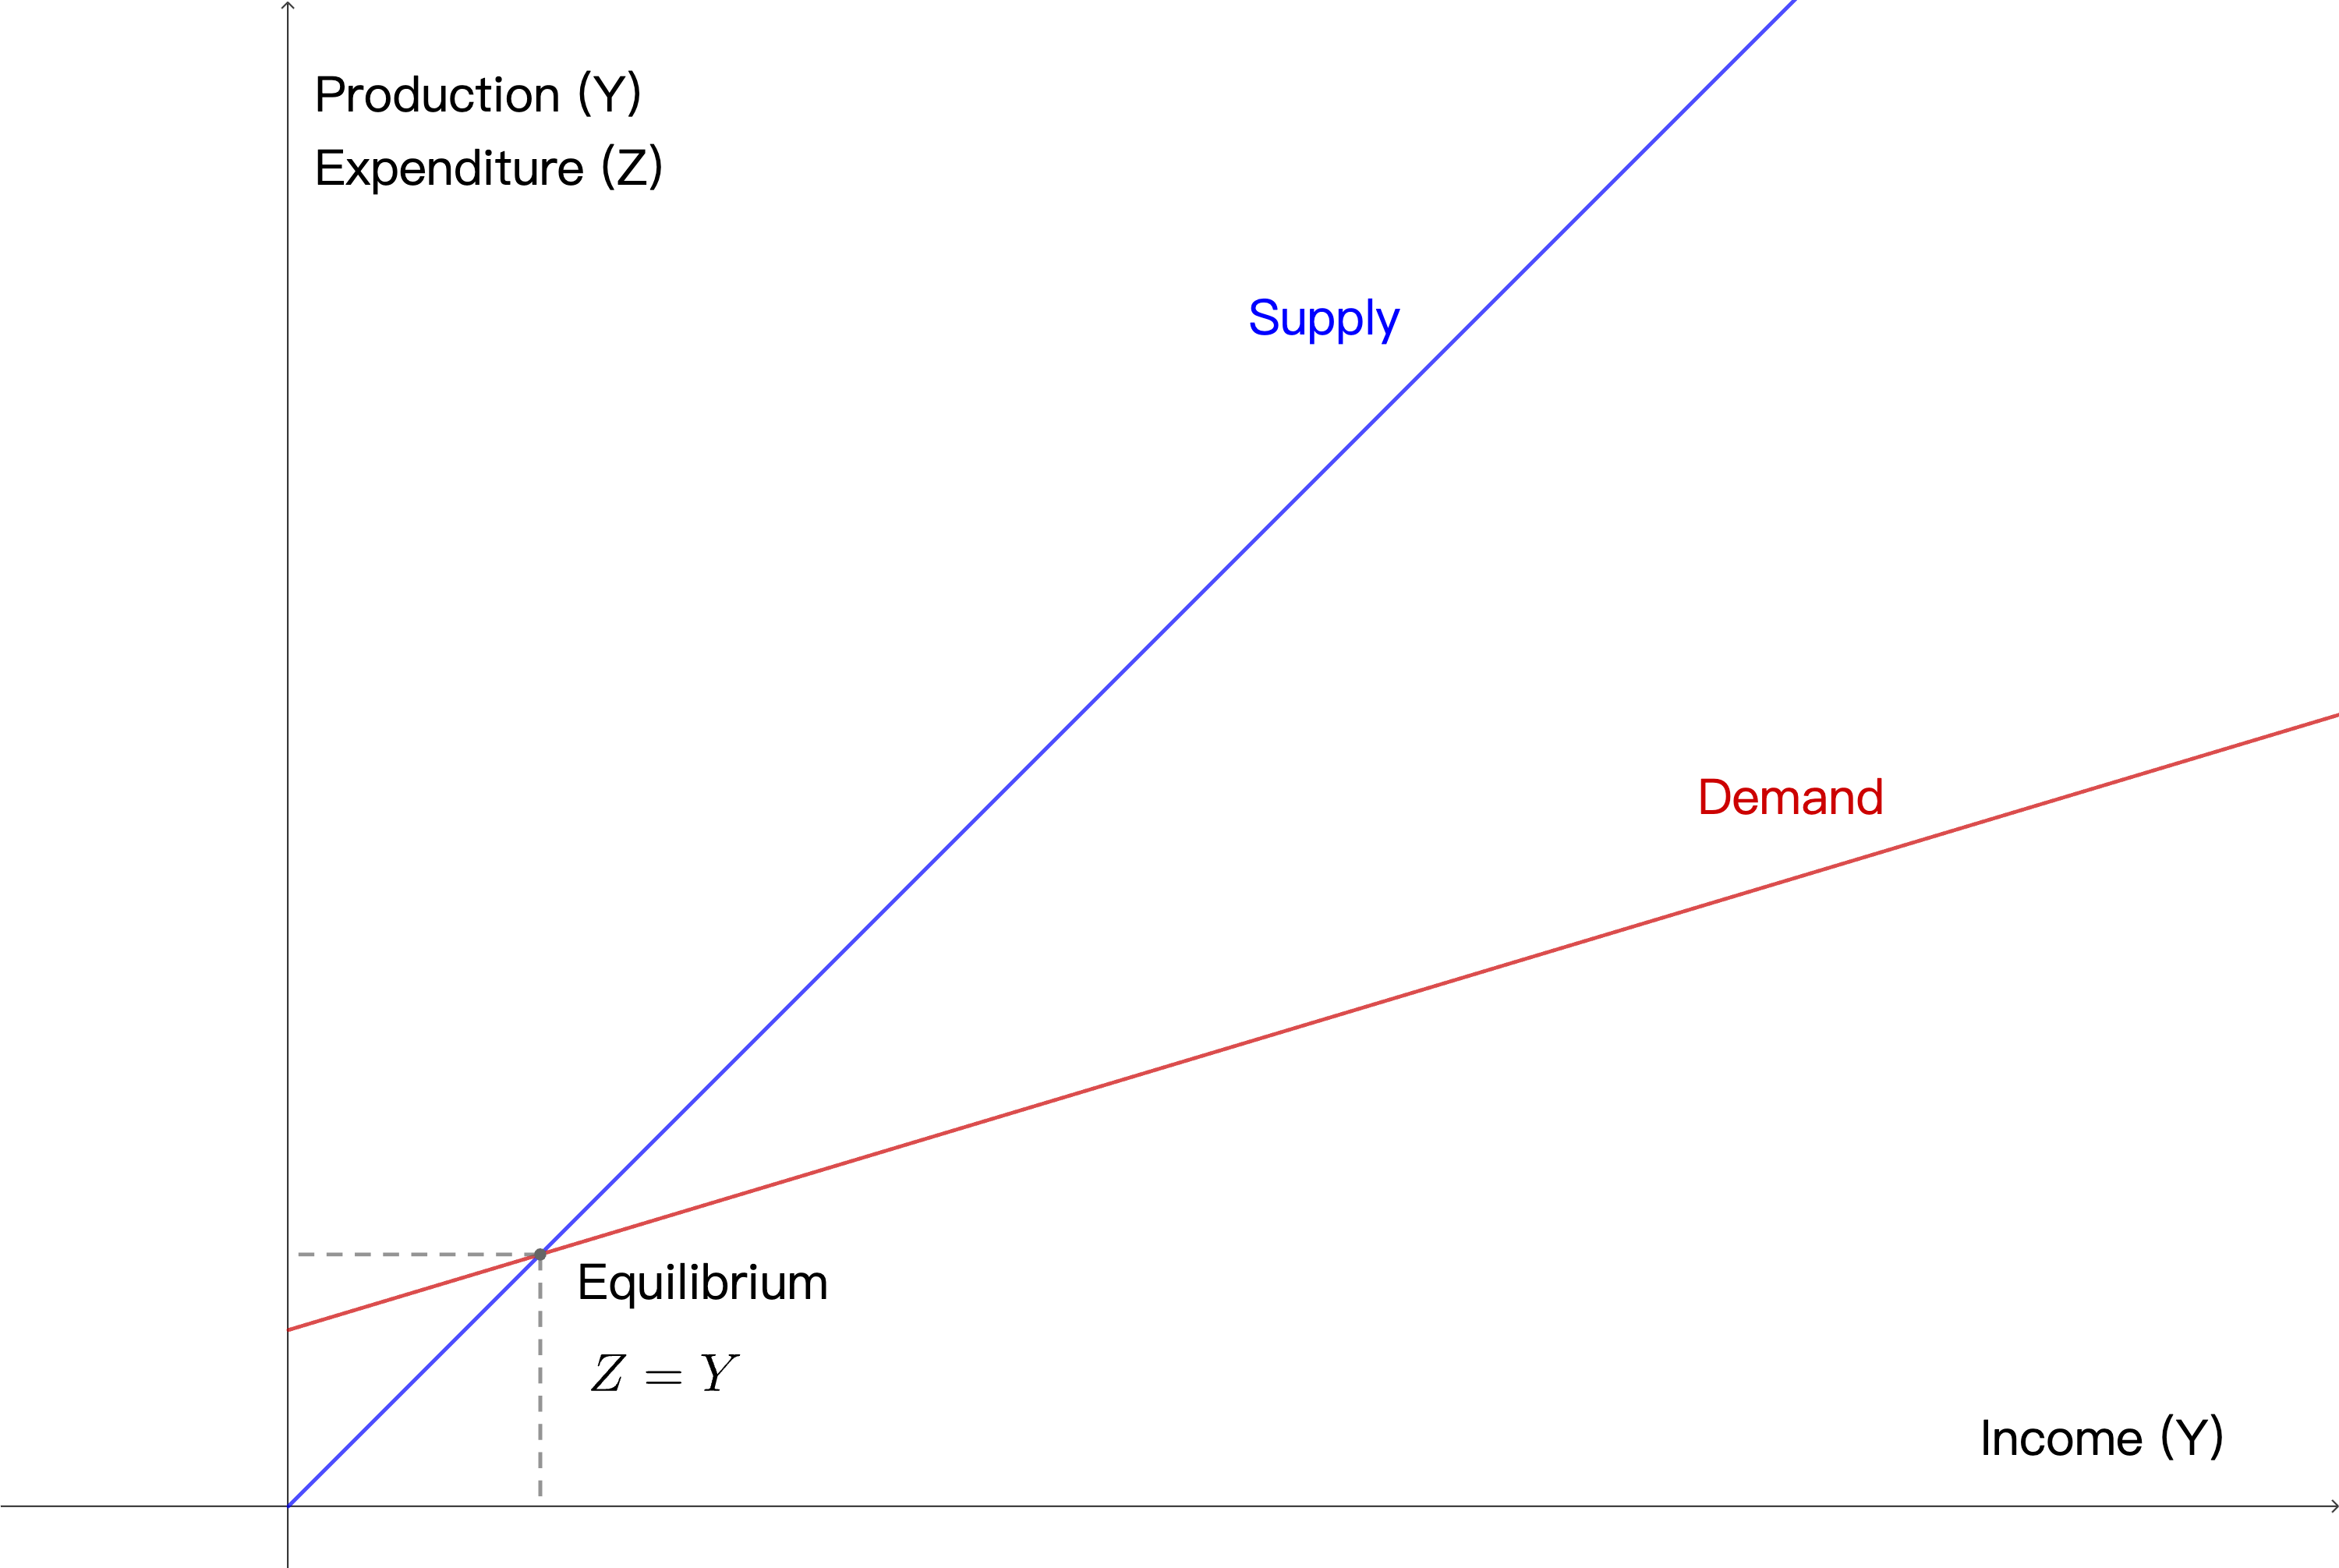
\includegraphics[width=0.8\textwidth]{keynesian_cross_0.png}
    \caption{Goods Market Equilibrium, Keynesian Cross}
    \label{fig:key_cross_v1}
\end{figure}

Figure \ref{fig:key_cross_v1} graphically shows the equilibrium. 
\begin{itemize}
    \item On the supply side, given income $Y$, we always have income equal to production. So it is the blue 45 degree line.
    \item On the demand side, we assume that $c_0 + \bar{I} + G - c_1T > 0$ and $c_1 > 0$. Since we typically have $c_1<1$ (why?), this ensures the existence of equilibrium.
\end{itemize}

\paragraph{Autonomous Spending and Multiplier}
Now consider increasing the autonomous consumption. This moves the demand line upward so that the equilibrium income and expenditure both increase. This is shown in Figure \ref{fig:key_cross_v2}.

\begin{figure}[htp]
    \centering
    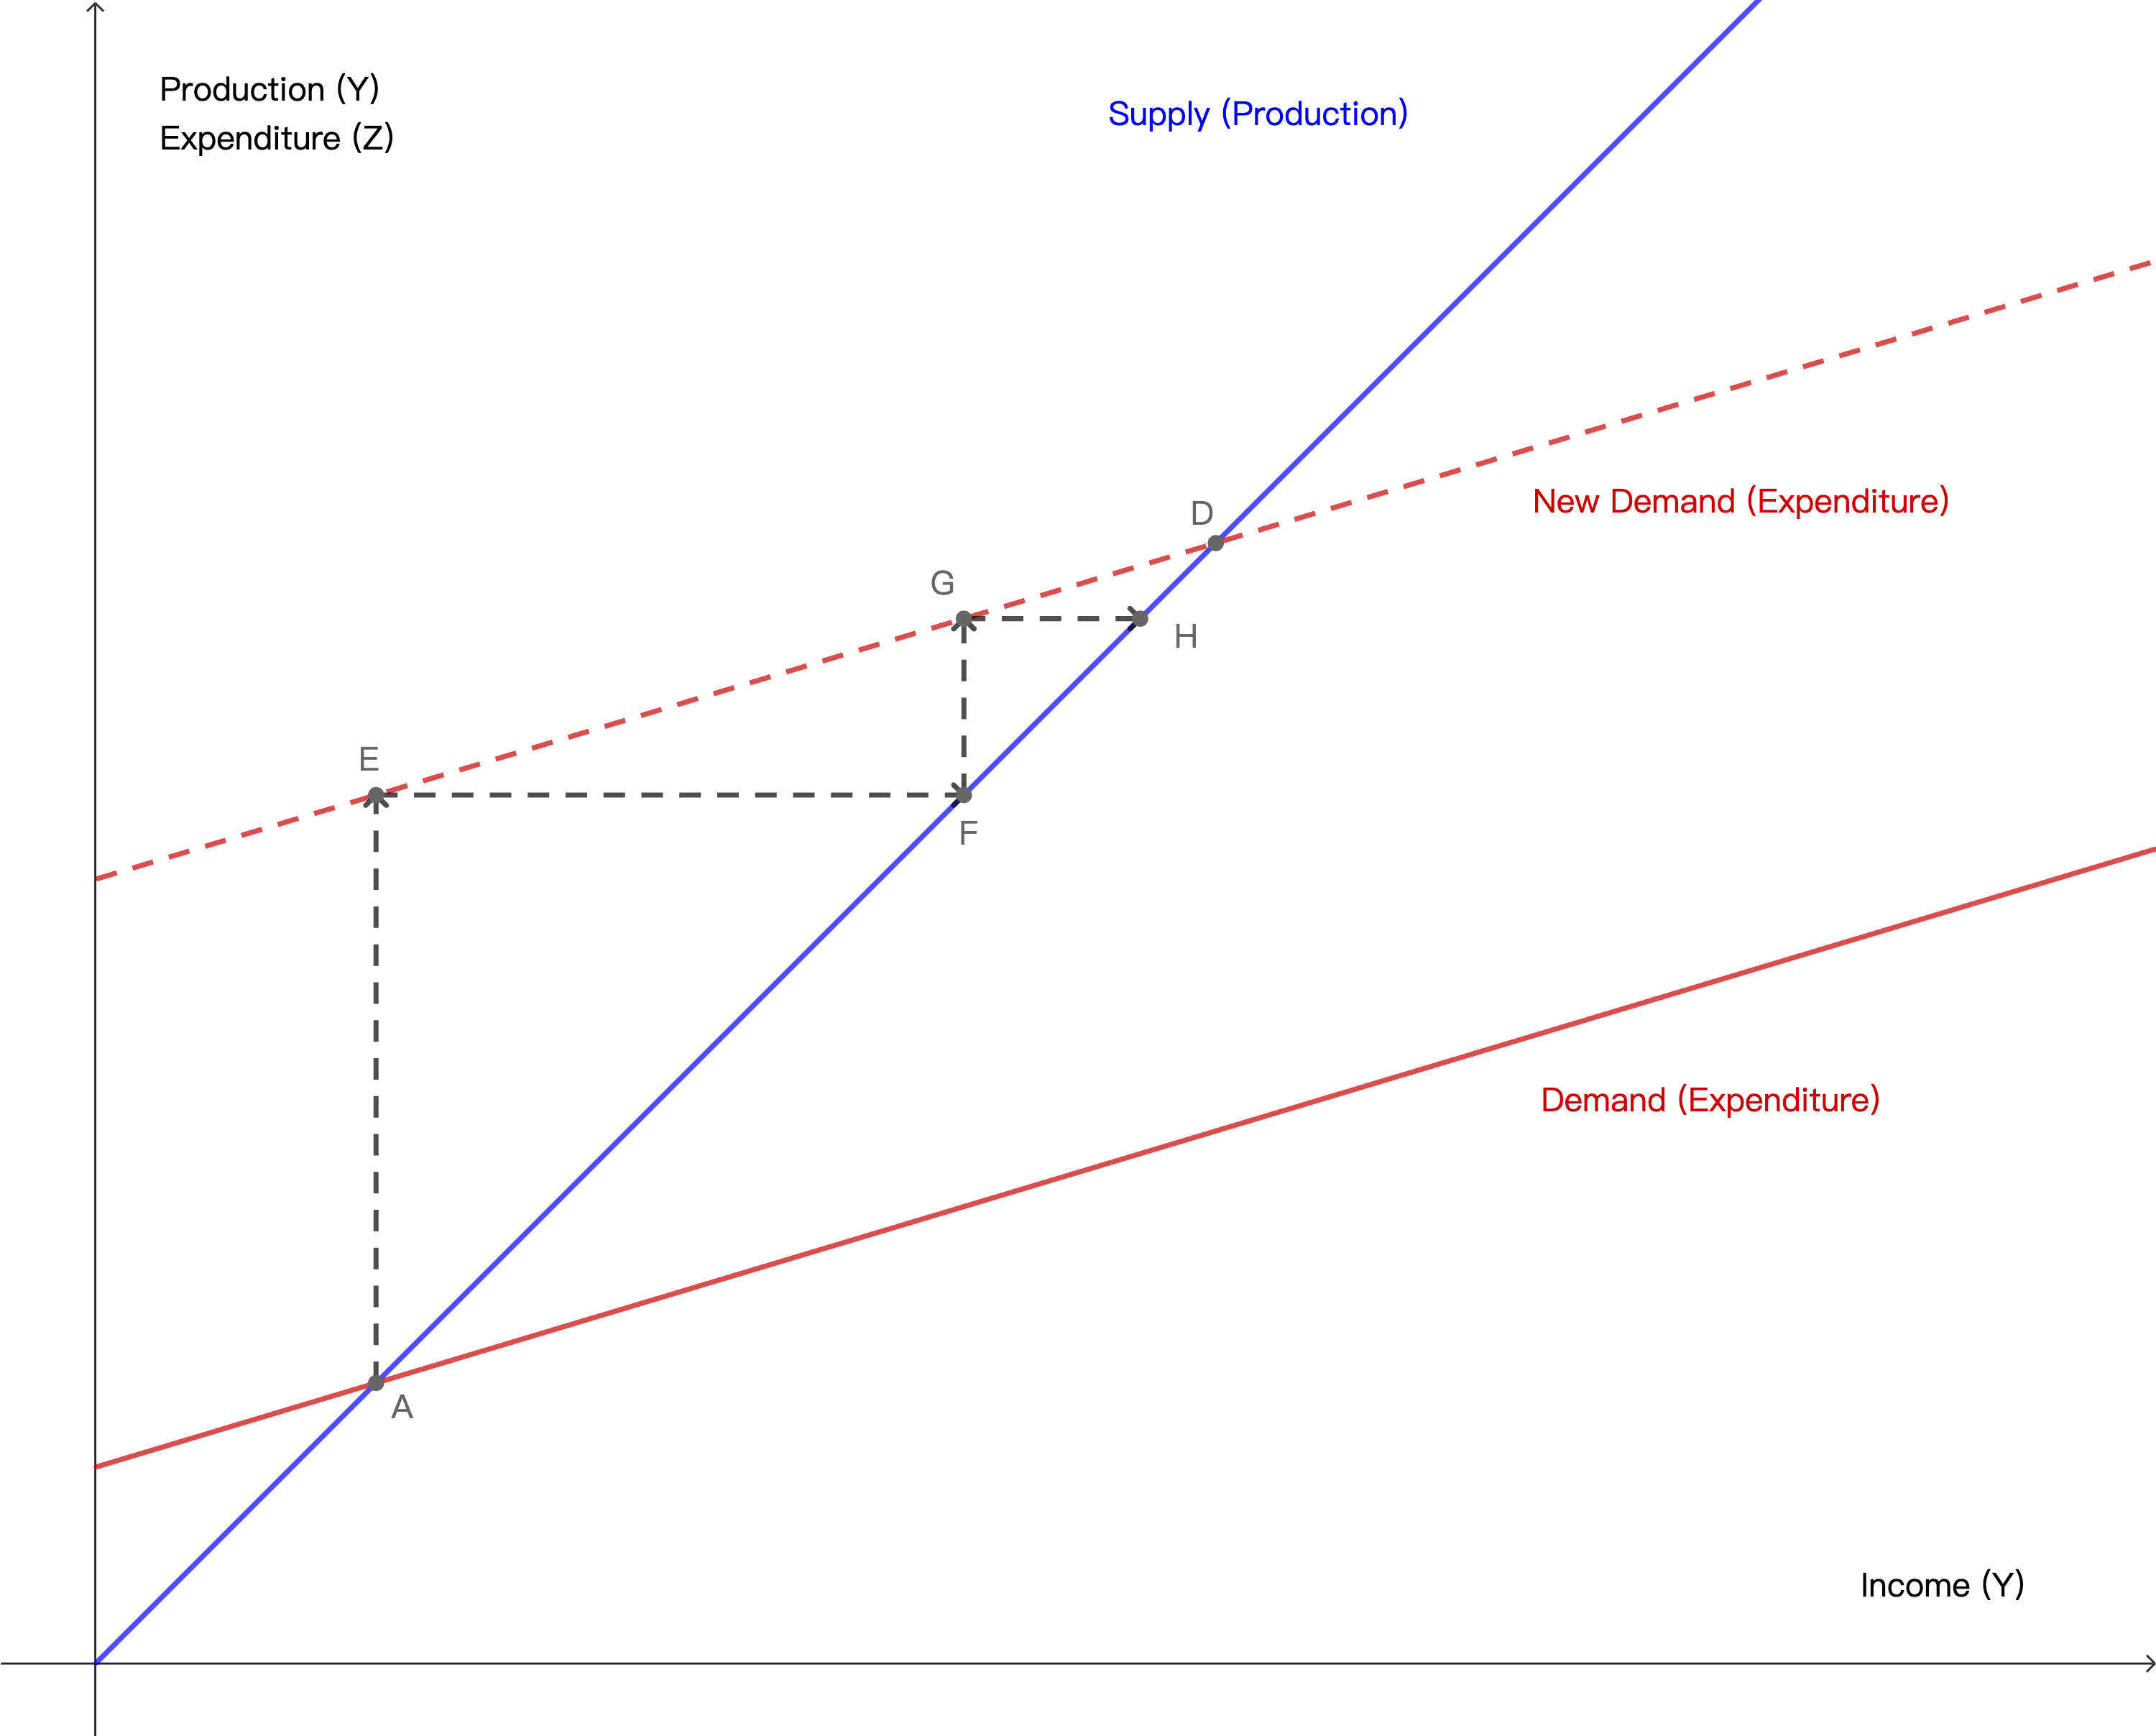
\includegraphics[width=0.8\textwidth]{keynesian_cross_c0change.png}
    \caption{Increasing $c_0$ moves demand upward}
    \label{fig:key_cross_v2}
\end{figure}

We would like to know how equilibrium output change from point $A$ to point $D$ when $c_0$ increases to $c_0'$. This idea is captured by the concept of \textbf{multiplier}. The multiplier implies how much output will increase given a unit increase in autonomous spending. 

Graphically, we can decompose the increase from $A$ to $D$ into multiple rounds. In the $n$-th round of increase, the output increases by $c_1^{n-1}$ unit. Summing up all the rounds, we get a geometric series:
\begin{align*}
    1 + c_1 + c_1^2 + \cdots + c_1^n + \cdots = \sum_{i=1}^{+\infty} c_1^{i-1} = \frac{1}{1-c_1}.
\end{align*}

Algebraically, substituting \eqref{eq:demand_v1} into \eqref{eq:eqm_cond}, we get
\begin{align*}
    Y = (c_0 + \bar{I} + G - c_1T) + c_1Y.
\end{align*}
This isequivalent to
\begin{align*}
    Y = \frac{1}{1-c_1} (c_0 + \bar{I} + G - c_1T).
\end{align*}
Holding other variables constant, if we inrease $c_0$ by 1 unit, then $Y$ increases by $\frac{1}{1-c_1}$ units.

\paragraph{MPC and Multiplier}
Figure \ref{fig:key_cross_v3} illustrates the change of equilibrium with two different demand lines that differ only in $c_1$, the marginal propensity to consumption. We notice that given a same amount of increase in the autonomous spending, the increase of equilibrium output is larger for demand line 2 whose MPC is larger.

\begin{figure}[htp]
    \centering
    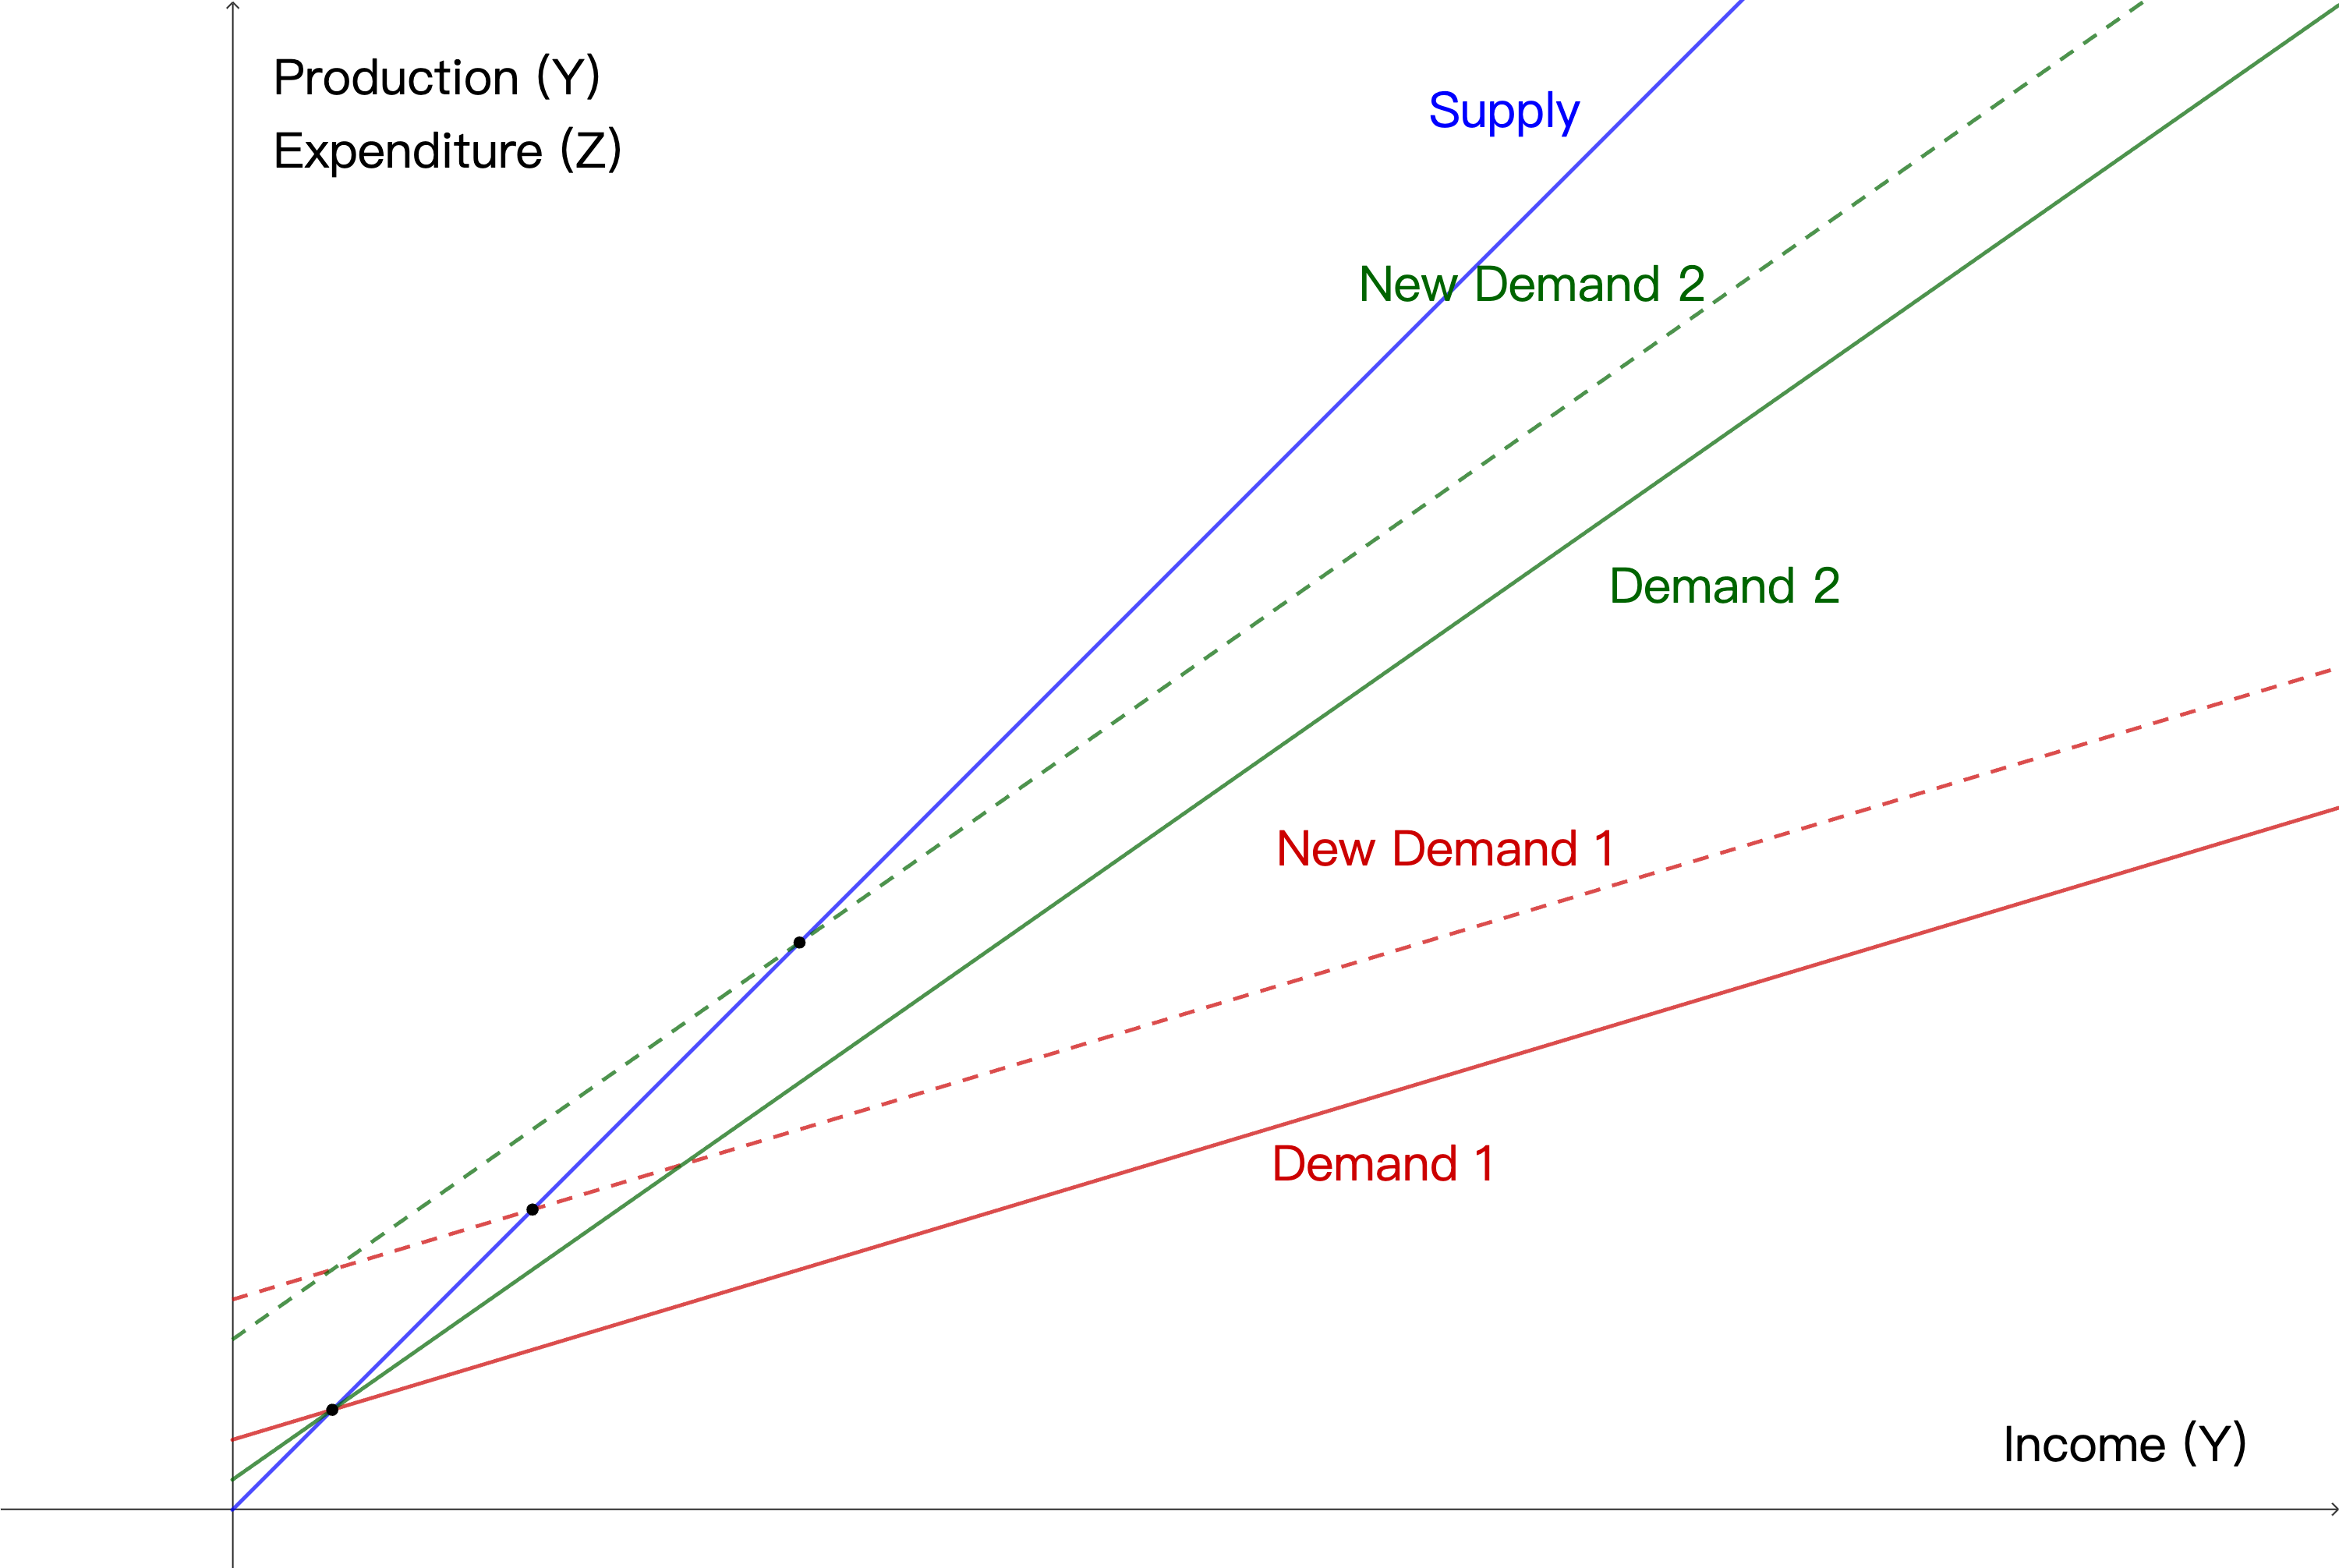
\includegraphics[width=0.8\textwidth]{keynesian_cross_c1change.png}
    \caption{Increasing $c_1$ yields larger multiplier}
    \label{fig:key_cross_v3}
\end{figure}

Algebraically, when $c_1$ increases, $\frac{1}{1-c_1}$ also increases.

\begin{exercise}
    Chapter 3, Question 2 in Blanchard, Olivier (2021), \textit{Macroeconomics}, 8th ed., Pearson.
\end{exercise}

\begin{example}
    Chapter 3, Question 5 (a)(b) and Question 6 (b) in Blanchard, Olivier (2021), \textit{Macroeconomics}, 8th ed., Pearson.

    [Words omitted.] Consider the following behavioral equations:
    \begin{align*}
        C &= c_0 + c_1Y_D\\
        T &= t_0 + t_1Y\\
        Y_D &= Y-T
    \end{align*}
    where $G$ and $I$ are constants. Assume that $t_1\in(0,1)$.
    \begin{enumerate}[label=\alph*.]
        \item Solve for the equilibrium output.
        \item What is the multiplier? Does the economy respond more to changes in autonomous spending when $t_1=0$ or $t_1>0$? Explain.
        \item Solve for taxes in equilibrium.
    \end{enumerate}
\end{example}

\vspace{36pt}

\begin{exercise}
    Chapter 3, Question 5 (c) and Question 6 (c)(d) in Blanchard, Olivier (2021), \textit{Macroeconomics}, 8th ed., Pearson.
\end{exercise}

\subsection*{Savings}
\paragraph{Private Saving and Public Saving}
\textbf{Private saving} equals disposable income minus consumption:
\begin{align}\label{eq:def_priv_s}
    S = Y_D - C = Y - T - C.
\end{align}
\textbf{Public saving} equals taxes (net of transfers) minus government spending:
\begin{align*}
    T - G
\end{align*}

\paragraph{Goods Market Equilibrium and IS relation}
By \eqref{eq:demand_v1} and \eqref{eq:eqm_cond}, the equilibrium condition can be rewritten as
\begin{align}\label{eq:eqm_cond_v2}
    Y = C + I + G.
\end{align}
Rewriting the condition, we get
\begin{align*}
    Y - T - C = I + G - T.
\end{align*}
Note that that left-hand side (LHS) of the equation is private savings $S$. Rearranging the temrs, we get the IS relation:
\begin{align*}
    I = S + (T-G),
\end{align*}
\textbf{I}nvestment equals \textbf{S}avings. More specifically, IS relation implies that at goods market equilibrium, the amount that firms want to invest must equal the amount that people and the government want to save.

As we have just shown, we can alternatively think about goods-market equilibrium as the condition that investment equals savings.

\paragraph{The Paradox of Saving}
Substituting the consumption function into \eqref{eq:def_priv_s}, we obtain
\begin{align*}
    S = -c_0 + (1-c_1)(Y-T).
\end{align*}
$1-c_1$ is called the \textbf{marginal propensity to save} (MPS).

What happens if we decrease saving by increasing $c_0$? You will deal with this in Problem Set.

\begin{exercise}
    When a person gets an increase in current income, what is likely to happen to consumption and saving?
    \begin{enumerate}[label=\Alph*.]
        \item Consumption increases and saving increases.
        \item Consumption increases and saving decreases.
        \item Consumption decreases and saving increases.
        \item Consumption decreases and saving decreases.
    \end{enumerate}
\end{exercise}

\begin{example}
    Consider an economy characterized by the following behavioral equations:
    \begin{align*}
        C &= c_0 + c_1 Y_D\\
        Y_D &= Y - T\\
        T &= t_1 Y + t_2 C
    \end{align*}
    where $t_1, t_2 \in (0,1)$. $G$ and $I$ are given. This is case when we tax both income and consumption. The economy is now at its equilibrium.
    \begin{enumerate}[label=(\arabic*)]
        \item Solve for the equilibrium output.
        \item What is the multiplier? Does this form of tax stabilizes output changes when there is a change in $c_0$, comparing with exogenous tax? Discuss cases where it does and it does not based on the equilibrium in part (1).
        \item Suppose that $c_0$ increases by 1 unit. In the new equibrlium, will consumption also increase by 1 unit? Discuss cases where it will and it will not based on the equilibrium in part (1).
        \item Write equilibrium saving as a function of $Y$.
        \item What is the MPS? Show that when $c_0$ increases by 1 unit, if $t_1+t_2=1$, the new equilibrium saving will decrease by 1 unit.
    \end{enumerate} 
\end{example}

\subsection*{Government and Fiscal Policy: Financial Stimulus}
Recall that at equilibrium, we have
\begin{align*}
    Y = \frac{1}{1-c_1}(c_0 + \bar{I} + G - c_1T).
\end{align*}
In the previous two examples, we have seen some ways to stabilize business cycles. Government can actually use financial stimulus to stabilize business cycle. Consider the following three alternatives:
\begin{enumerate}[label=(\arabic*)]
    \item Increase government spending by 1 unit while holding other accounts constant.
    
    Recall that we are in the equilibrium, so
    \begin{align*}
        Y = Z = C + I + G.
    \end{align*}
    We also have the following behavioral equation:
    \begin{align*}
        C = c_0 + c_1(Y-T).
    \end{align*}
    If $G$ increases by 1 unit, then $Y$ increases by 1 unit, so $C$ increases by $c_1$ unit. This takes effect again in the equilibrium condition, which lets $Y$ increase by $c_1$ more unit, thus $C$ increase by $c_1 \times c_1 = c_1^2$ unit. Continue with the process, the \textbf{spending multiplier} will be
    \begin{align*}
        \frac{\Delta Y}{\Delta G} = \frac{\sum_{i=0}^{+\infty}c_1^i}{1} = \frac{1}{1-c_1}.
    \end{align*}
    \item Decrease tax by 1 unit while holding other accounts constant.
\end{enumerate}
\end{document}